\documentclass[__main__.tex]{subfiles}

\begin{document}

\section{Принцип замороженных коэффициентов, примеры использования этого принципа для одномерного параболического уравнения с переменным коэффициентом диффузии}

Принцип замор. коэфф. рассм. на примере ур-я диффузии с перем. коэфф. диффузии (D) рассмотрим задачу Коши:

\begin{equation} \label{42.1}
\begin{cases}
\frac{\partial U}{\partial t} - a(x,t) \cdot \frac{\partial^2 U}{\partial x^2} = 0, \ \left(x,t\right) \in \mathbb{R} \times \left(0,T\right) \\
U(x,t) = \mu(x), \ x\in [a;b], \ t \in \textbf{[0;T]} \\
U(a,t) = \beta_1(x), \ U(b,t) = \beta_2(x)
\end{cases}
\end{equation}

\paragraph{}
Для численного решения задачи (1) вводим двумерную сетку C = A x B = ($x_k, t^n$): $n = \overline{0,N}, k = \overline{0,K}$  A = <$0 = t_0, t_1 .. t_N $>, B = <$a = x_0, x_1 .. x_m $> - равномерная сетка шагов $\tau$ = stp(B) и h = stp(A). Тогда явный разностный аналог задачи (1):

\begin{figure}[ht]
	\centering
	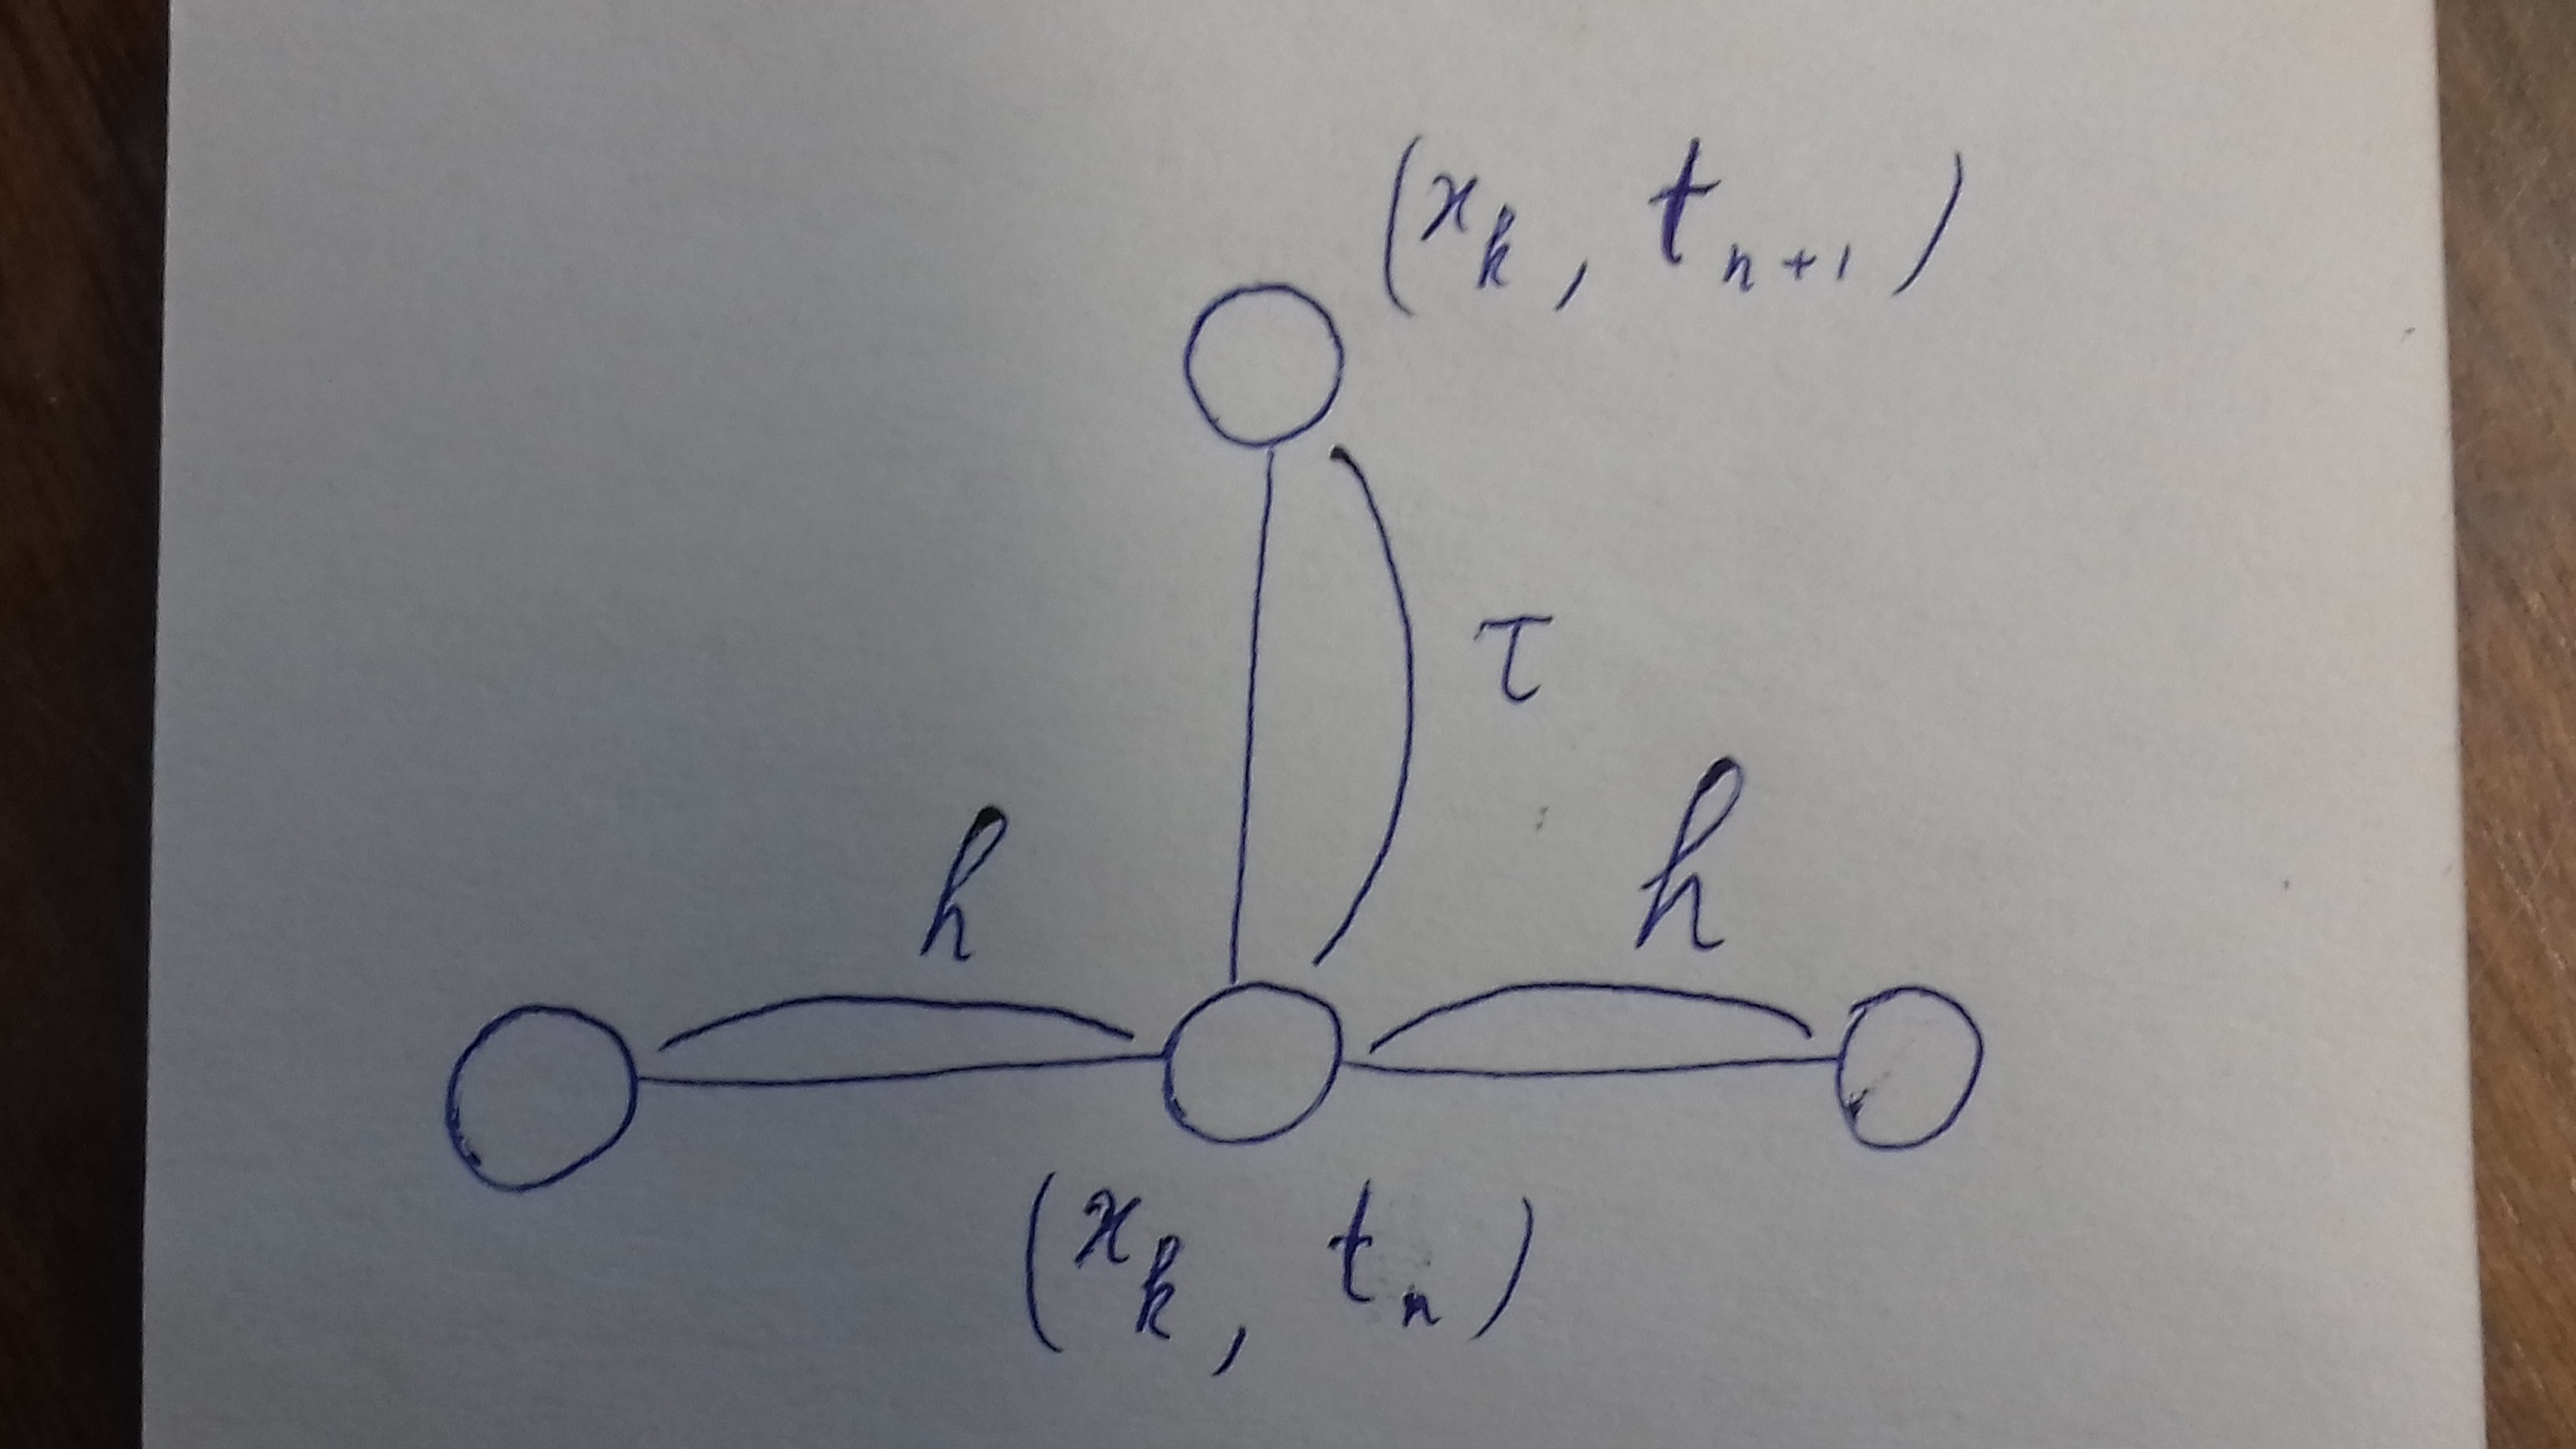
\includegraphics[width=0.4\linewidth]{img/img_42_1}
	\caption{}
	\label{img_42.1}
\end{figure}

\begin{equation} \label{42.2}
\begin{cases}
\frac{U^{n+1}_k - U^{n}_k}{\tau} - a^n_k \frac{U^{n}_{k-1} - 2U^{n}_k + U^n_{k+1}}{h^2} = 0, \\
U^0_k = \mu_k, k = \overline{1,K-1} \\
U^n_0 = \beta_1^n \textbf{и}, n = \overline{0,N-1} \\
U^n_k = \beta_2^n \textbf{и}, n = \overline{1,N} 
\end{cases}
\end{equation} 

Заморозим коэффициент $a^n_k$ около $x_k$. Для устойчивости схемы (2):

$$
\frac{2\tau \cdot max ({a^n_k: n = \overline{0,N}, k = \overline{0,K}})}{h^2} < 1.
$$

\paragraph{Принцип замороженных коэффициентов}

Коэффициент a "замораживается" во внутренних точках сетки С (сетка С должна быть достаточно подробной), т. е. предполагается, что в ближайшем к внутреннему узлу в межузельном пространстве коээфициент a - постоянный. После такого предположения считается, что в разностном аналоге задачи используются постоянные коэффициенты.

Мы помним, что параметр Курранта 


$\text{\ae} = $$\frac{\tau}{h^2}$, 

тогда получаем:

\begin{equation} \label{42.3}
U^{n+1}_k = \text{\ae} \cdot a^n_k \cdot U^n_{k-1} + (1 - 2a^n_m \text{\ae})U^n_k + \text{\ae} \cdot a^n_k \cdot U^n_{k+1}
\end{equation}

Согласно (необходимому) спектральному признаку для $\forall n, m$ должно вып-ся следующее условие (можно использовать признак для монотонных схем):

\begin{equation} \label{42.4}
2a^n_k \cdot \text{\ae} \leq 1,  n = \overline{0,N-1},  k = \overline{1,K-1}
\end{equation}

Следовательно, спектральный признак выполняется при

\begin{equation} \label{42.5}
2 \text{\ae} \cdot max \{( a(x,t): (t,x) \in[o;T] x [a;b])\} \leq 1
\end{equation}

Принцип замороженных коэфф. может быть использован для нелинейных задач. В качестве примера рассмотрим нелинейную задачу. В этом случае приходится менять шаг сетки для разных временных слоев.

\begin{equation} \label{42.6}
\begin{cases}
\frac{\partial U}{\partial t} - a(x,t) \cdot \frac{\partial^2 U}{\partial x^2} = 0, \ \left(x,t\right) \in \mathbb{R} \times \left(0,T\right) \\
U(x,t) = \mu(x), \ x\in [a;b], \ t \in \textbf{[0;T]} \\
U(a,t) = \beta_1(x), \ U(b,t) = \beta_2(x)
\end{cases}
\end{equation}

Для явного разностного аналога при $n \in \textbf{<0;N-2>}$ из задачи (6) получаем 

\begin{equation} \label{42.7}
\frac{U^{n+1}_k - U^{n}_k}{\tau_n} - (1 + (u^n_k)^2)\frac{U^{n}_{k-1} - 2U^{n}_k + U^n_{k+1}}{h^2} = 0,
\end{equation} 

Введем обозначение:
 \begin{equation} \label{42.8}
 \begin{cases}
 a^n_k = 1 + (u^n_k)^2, \\
 \text{\ae} = \frac{\tau_n}{h^2_k}
 \end{cases}
 \end{equation} 
 
Тогда:

 \begin{equation} \label{42.9}
U^{n+1}_k = a^n_k \cdot \text{\ae}_n \cdot U^n_{k-1} + (1 - 2a^n_m \text{\ae})U^n_k + \text{\ae} \cdot a^n_k \cdot U^n_{k+1}
\end{equation} 
 
 Для выполнения спектрального признака:
 
 \begin{equation} \label{42.10}
 \begin{cases}
  2a^n_k \cdot \frac{\tau_n}{h^2_k} \leq 1, k = \overline{1,K-1}, \Rightarrow \\
  2max \{((1 + a^n_k)^2:  k = \overline{0,K})\} \cdot \frac{2\tau_n}{h^2} < 1.
  \end{cases}
 \end{equation} 
 
 Следовательно:
 
 \begin{equation} \label{42.11}
 \tau_n \leq \frac{h^2}{2max \{(1 + a^n_k)^2:  k = \overline{0,K}\}}
 \end{equation} 
 
 где $U^n_0, U^n_1 ... U^n_k$ - найдены для слоя n, $n = \overline{0,N-2}$
 
\end{document}
